%% LaTeX2e class for student theses
%% thesis.tex
%% 
%% Based on SDQ KIT Template by Erik Burger
%%
%% Karlsruhe Institute of Technology
%% Institute for Automation and Applied Informatics
%% AIDA Research Group
%%
%% Nicole Ludwig
%% nicole.ludwig@kit.edu
%%
%% Version 1.2, 2018-10-11

%% Available page modes: oneside, twoside
%% Available languages: english, ngerman
%% Available modes: draft, final
\documentclass[twoside,english, 12pt]{thesisIAI}

%% ---------------------------------
%% | Additonal Packages |
%% ---------------------------------
\usepackage{amsmath}
\usepackage{amsfonts}
\usepackage{amssymb}
\usepackage{pdfpages}
\usepackage{booktabs}
\usepackage{siunitx}
\usepackage[utf8]{inputenc}
\usepackage{footnote}
\usepackage{tocloft}
\usepackage{hyperref}

\usepackage{graphicx}
\usepackage{epstopdf}

\usepackage{transparent}
\usepackage{color}
\graphicspath{{figure/}}



\usepackage{tocbasic}
\usepackage{caption}

%%% Doc: ftp://tug.ctan.org/pub/tex-archive/macros/latex/contrib/caption/caption.pdf
\usepackage{caption}
% Aussehen der Captions
\captionsetup{
   margin = 10pt,
   font = {rm},
   labelfont = {bf},
   format = plain, % oder 'hang'
   indention = 0em,  % Einruecken der Beschriftung
   labelsep = space, %period, space, quad, newline
   justification = RaggedRight, % justified, centering
   singlelinecheck = true, % false (true=bei einer Zeile immer zentrieren)
   position = bottom %top
}


%%% Bugfix Workaround
\DeclareCaptionOption{parskip}[]{}
\DeclareCaptionOption{parindent}[]{}
 

\usepackage{csquotes}
\usepackage{cleveref}
\usepackage{siunitx}

%% useful abreviations

\newcommand\ie{i.\,e.\xspace}
\newcommand\eg{e.\,g.\xspace}
\newcommand\Eg{E.\,g.\xspace}
\newcommand\NB{N.\,B.\xspace}
\newcommand\BSc{B.\,Sc.\xspace}
\newcommand\MSc{M.\,Sc.\xspace}
\newcommand\PhD{Ph.\,D.\xspace}
\newcommand\etc{etc.\xspace}
\newcommand\cf{cf.\xspace}
\newcommand\Cf{Cf.\xspace}
\newcommand\etal{et\,al.\xspace}
\newcommand\page[1]{p.\,#1}
\newcommand\pages[1]{pp.\,#1}
\newcommand\ham{a.\,m.\xspace}
\newcommand\hpm{p.\,m.\xspace}
	
\newcommand\zB{z.\,B.\xspace}
\newcommand\proz{\,\%\xspace}

%% von mir hinzugefügt

\usepackage{color}
\usepackage{transparent}
\graphicspath{{figure/}}


%% ---------------------------------
%% | Information about the thesis  |
%% ---------------------------------

%% Name of the author
\author{Vivien Geenen}

%% Title (and possibly subtitle) of the thesis
\title{Model- Predictive Control of Heat Pump in Smart Buildings}

%% Type of the thesis 
\thesistype{Master's thesis}
%\thesistype{Seminar Paper}

%% Change here the faculty 
%\faculty{Seminar}
\faculty{Engineering}
%\faculty{Informatics}

%% The advisors are PhDs or Postdocs
\advisorone{Moritz Frahm, M.Sc. and Frederik Zahn, M.Sc}

%% The second advisor can be omitted
%\advisorone{}

%% Please enter the start end end time of your thesis
\editingtime{June}{November 2021}

\settitle

%% Please do not change anything in this tex file without talking to your supervisor
%% LaTeX2e class for student theses
%% format.tex
%% 
%% Based on SDQ KIT Template by Erik Burger
%%
%% Karlsruhe Institute of Technology
%% Institute for Automation and Applied Informatics
%% AIDA Research Group
%%
%% Nicole Ludwig
%% nicole.ludwig@kit.edu
%%
%% Version 1.2.1, 2018-10-11

%% This file switches between the official reviewers and addresses of the faculties 

\ifthenelse{\equal{\thefaculty}{Seminar}}{\uppertitleback}{\ifthenelse{\equal{\thefaculty}{Engineering}}{\uppertitleback{Karlsruher Institut für Technologie\\ Fakultät für Maschinenbau\\ Postfach 6980\\ 76128 Karlsruhe}}{\uppertitleback{Karlsruher Institut für Technologie\\ Fakultät für Informatik\\ Postfach 6980\\ 76128 Karlsruhe}}}


\ifthenelse{\equal{\thefaculty}{Engineering}}{\reviewerone{Prof. Dr. Veit Hagenmeyer}}{\reviewertwo{apl. Prof. Dr. Jörg Matthes}}

\ifthenelse{\equal{\thefaculty}{Seminar}}{\reviewertwo{}}{\ifthenelse{\equal{\thefaculty}{Informatics}}{\reviewertwo{Prof. Dr. Achim Streit}}{\reviewertwo{apl. Prof. Dr. Jörg Matthes}}}

\ifthenelse{\equal{\thefaculty}{Seminar}}{\facultyname{Energy Informatics Seminar}}{\ifthenelse{\equal{\thefaculty}{Engineering}}{\facultyname{\iflanguage{english}{at the Department of Mechanical Engineering}{an der Fakultät für Maschinenbau}}}{\facultyname{\iflanguage{english}{at the Department of Informatics}{an der Fakultät für Informatik}}}}

%% --------------------------------
%% | Settings for word separation |
%% --------------------------------

%% Describe separation hints here.
%% For more details, see 
%% http://en.wikibooks.org/wiki/LaTeX/Text_Formatting#Hyphenation
\hyphenation{
% me-ta-mo-del
}

%% --------------------------------
%% | Bibliography                 |
%% --------------------------------

% Please make sure your bibfiles name is thesis.bib and is located in the tex subfolder
\usepackage[                 % !! what about the ``biblatex.cfg''?
        backend=bibtex8,      % (bibtex), bibtex8, biber
%        %
        style=numeric-comp,		 %numeric-comp,authoryear
%        bibstyle=,          % should not be used without citestyle and vice versa
%        citestyle=,
%        natbib=true,
        %
%        sorting=nty,        % (nty), nyt, nyvt, anty, anyt, anyvt, debug, none
%        sortlos=los,        % bib, (los)
%        sortcites=false,    % false
%        maxnames=2,         % <integer> (3)
				maxcitenames=2,      % sets the maximum numbers of authors before abbreviated to et al in text
				maxbibnames=25,       % sets the maximum numbers of authors before abbreviated to et al in bibliography
%        minnames=1,         % (1)
%        maxitems=3,         % (3)
%        minitems=1,         % (1)
%        autocite=,          % inline, footnote, superscript, ...
%        autopunct=true,     % true
%        babel=none,         % (none), hyphen, other, other*
%        block=none,         % (none), space, par, nbpar, ragged
        hyperref=true,      % false
%        backref=false,      % false
%        indexing=false,     % true, (false), cite, bib
%        refsection=none,    % (none), part, chapter, section, subsection
%        refsegment=none,    % (none), part, chapter, section, subsection
%        citereset=none,     % (none), part, chapter, section, subsection
%        abbreviate=true,    % true
%        date=long,          % short, (long)
%        urldate=short,      % (short), long
%        defernums=false,    % false
%        punctfont=false,    % false
        %
%        mincrossrefs=2,     % 2
        bibencoding=inputenc,   % (ascii), inputenc, <encoding>
        %%
%        keywsort=false,     % false
    %
%     useauthor=false,   % true
%     useeditor=false,   % true
%        useprefix=true,     % false
    %
%        pagetracker=true,   % true, (false), page, spread
%     citetracker=true,   % true, (false), context, strict, constrict
%     ibidtracker=true,   % true, (false), context, strict, constrict
%     opcittracker=true,   % true, (false), context, strict, constrict
%     loccittracker=true, % true, (false), context, strict, constrict
%        terseinits=true,    % false
%     labelalpha=true,   % false
%     labelnumber=true,   % false
%     labelyear=true,   % false
%     singletitle=true,   % false
      uniquename=init,   % true, (false), init
%
        doi=false,
        url=false,
				isbn = false,
        giveninits = true % render first/middle names as initals
            ]{biblatex}
	
\makeatletter
\def\blx@maxline{77}
\makeatother
	
	\bibliography{tex/thesis}
   
      %  \DefineBibliographyStrings{ngerman}{%
         %   bibliography     = {Literaturverzeichnis},  % = \bibname
         %   references       = {Literatur},             % = \refname
     %   }
        \defbibnote{alphabetic}{%
            Die Literaturangaben sind alphabetisch nach den Namen
            der Autoren sortiert. Bei mehreren Autoren wird nach
            dem ersten Autor sortiert.\par
            Und mit dem neuen \LPack{biblatex}-Paket funktioniert
            das auch, wie man unschwer erkennen kann.\par\bigskip
        }

% -------------------------------------------------------------------------------------------------
%% declare author names as "last, first".
%% Either for the first author only or for all authors
%\DeclareNameFormat{author}{%
%    \ifthenelse{\value{listcount}=1}
%        {#1%                                            % first author
%            \ifblank{#3}{}{\addcomma\space #3}}
%        {#1%                                            % all the other authors (last, first)
%            \ifblank{#3}{}{\addcomma\space #3}}%
%%        {\ifblank{#3}{}{#3\space}%                      % all the other authors (first last)
%%            #1}%
%    \ifthenelse{\value{listcount}<\value{liststop}}
%        {,\space}
%            {}
%}
%
%%http://projekte.dante.de/DanteFAQ/BiblatexReihenfolgeAutoren
%\DeclareNameFormat{last-first}{%
%  \iffirstinits
%    {\usebibmacro{name:last-first}{#1}{#4}{#5}{#7}}
%    {\usebibmacro{name:last-first}{#1}{#3}{#5}{#7}}%
%  \usebibmacro{name:andothers}}
%\DeclareNameFormat{labelname}{%
%   \ifuseprefix
%     {\usebibmacro{name:last-first}{#1}{#4}{#5}{#8}}
%     {\usebibmacro{name:last-first}{#1}{#4}{#6}{#8}}%
%   \usebibmacro{name:andothers}}

%  \DefineBibliographyStrings{english}{%
%    typeeditor = {{}{}},
%    typeeditors = {{}{}},
%    in = {{}{}},
%    inseries = {{}{}},
%    byeditor = {{}{}}
%  }

%-------------------------------------------------------------------------------------------------

%% http://www.golatex.de/biblatex-anpassen-die-x-te-frage-t4657.html
\renewbibmacro*{journal+issuetitle}{%
  \usebibmacro{journal}%
  \setunit*{\addcomma\space}%
  \iffieldundef{series}
    {}
    {\newunit
     \printfield{series}%
     \setunit{\addcomma\space}}%
  \printfield{volume}%
  \setunit*{\addcomma\space}%
  \printfield{number}%
  \setunit{\addcomma\space}%
  \printfield{eid}%
  \setunit{\addspace}%
  \usebibmacro{issue+date}%
  \setunit{\addcolon\space}%
  \usebibmacro{issue}%
  \newunit}

\DeclareFieldFormat[article]{volume}{\bibstring{jourvol}~#1}
\DeclareFieldFormat[article]{number}{\bibstring{number}~#1} 
%\DeclareFieldFormat[article]{edition}{\bibstring{edition}~#1} 

%% http://mrunix.de/forums/showthread.php?t=67386
\DefineBibliographyStrings{english}{jourvol={Vol\adddot}} 
\DefineBibliographyStrings{english}{number={No\adddot}} 
\DefineBibliographyStrings{english}{edition={Ed\adddot}} 

\AtBeginBibliography{%
  % Setzt die Autoren-Vornamen auf Kapitälchen 
  \renewcommand*{\mkbibnamefirst}{\textsc}
  \renewcommand*{\mkbibnamelast}{\textsc}
  \renewcommand*{\mkbibnameprefix}{\textsc}
  \renewcommand*{\mkbibnameaffix}{\textsc}
  
  %%Doppelpunkt nach Namen, kein Punkt
  %\renewcommand*{\labelnamepunct}{\addcolon\space} 
  
  \DeclareFieldFormat{name}{\textsc{#1\isdot}}
  \DeclareFieldFormat{title}{\mkbibemph{#1\isdot}}
  
  %%\DeclareFieldFormat[article]{title}{#1}
  %%\DeclareFieldFormat[article]{title}{\mkbibquote{#1}}
  \renewcommand*{\mkbibquote}[1]{\mkbibemph{#1\isdot}}
 
  % http://tex.stackexchange.com/ ...
  % questions/16716/spell-out-volume-and-edition-in-words-biblatex-in-german
  %\renewcommand*{\mkbibordedition}[1]{\Ordinalstringnum{#1}[f]}
  \renewcommand*{\mkbibordedition}[1]{\ordinalnum{#1}}
} 

%% Set PDF metadata, must be set BEFORE \begin{document}
\setpdf

%% ====================================
%% ====================================
%% ||                                ||
%% || Beginning of the main document ||
%% ||                                ||
%% ====================================
%% ====================================
\begin{document}

\hypersetup{pageanchor=false}

%% Set the title
\maketitle

%% The Preamble begins here
\frontmatter

%% LaTeX2e class for student theses: Declaration of independent work
%% sections/declaration.tex
%% 
%% Karlsruhe Institute of Technology
%% Institute for Program Structures and Data Organization
%% Chair for Software Design and Quality (SDQ)
%%
%% Dr.-Ing. Erik Burger
%% burger@kit.edu
%%
%% Version 1.3.2, 2017-08-01

\thispagestyle{empty}
\null\vfill
\noindent\hbox to \textwidth{\hrulefill} 
\iflanguage{english}{I declare that I have developed and written the enclosed
\ifthenelse{\equal{\thefaculty}{Engineering}}{thesis}{\ifthenelse{\equal{\thefaculty}{Informatics}}{thesis}{paper}} completely by myself, and have not used sources or means without
declaration in the text.}%
{Ich versichere wahrheitsgemäß, die Arbeit
selbstständig angefertigt, alle benutzten Hilfsmittel vollständig und genau
angegeben und alles kenntlich gemacht zu haben, was aus Arbeiten anderer
unverändert oder mit Änderungen entnommen wurde.}
 
 
%% ---------------------------------------------
%% | Replace PLACE and DATE with actual values |
%% ---------------------------------------------
\textbf{Karlsruhe, 14. December 2021}
\vspace{1.5cm}
 
\dotfill\hspace*{8.0cm}\\
\hspace*{2cm}(\theauthor) 
\cleardoublepage

\setcounter{page}{1}
\pagenumbering{roman}

%% ----------------
%% |   Abstract   |
%% ----------------
 
%% For theses written in English, an abstract both in English
%% and German is mandatory.
%%
%% Seminar Papers written in English need only an English abstract.
%%
%% For theses written in German, a German abstract is sufficient.
%%
%% The text is included from the following files:
%% - sections/abstract
%% - sections/zusammenfassung
\chapter{Kurzfassung}
\label{ch:kurzfassung}

\pdfbookmark[1]{Abstract}{Abstract}

\chapter{Abstract}

%\begin{center}
%  \begin{minipage}{12cm}
%    \begin{sloppypar}
%		As the share of electricity from regenerative sources is growing constantly, the weather becomes an increasingly important factor in the analysis of electricity markets. Hence, this thesis uses local weather data to predict electricity spot prices. More precisely, we include wind speed and temperature from individual German weather stations into time series and statistical learning models. However, as the available weather information is vast and renewable power is not generated everywhere, we use random forests and Bayesian structural time series to perform a feature selection. Overall, we manage to improve our forecasting accuracy of the EPEX electricity prices by up to \SI{7.69}{\percent} in terms of root mean squared error and up to \SI{8.19}{\percent} in terms of mean absolute error.
%    \end{sloppypar}
%  \end{minipage}
%\end{center}

\newpage

\hypersetup{pageanchor=true}
%% ------------------------
%% |   Table of Contents  |
%% ------------------------
\tableofcontents
\listoffigures
\listoftables
\setcounter{secnumdepth}{5}
\setcounter{tocdepth}{5}

%% -----------------
%% |   Main part   |
%% -----------------

\mainmatter

\chapter{Introduction}
\label{ch:introduction}
Climate change is challenging the entire world. In the Paris Agreement, the United Nations (UN) agrees to keep the rise in global average temperature significant under two degrees Celsius \cite{UnitedNations.2015}. To achieve this aim every nation has to reduce its greenhouse gas emissions. This calls for changes in the mobility sector, industry, and energy production, for example. Germany intends to implement this by promoting electromobility, using hydrogen in industry, and energy transition \cite{Deutschlandfunk.24.06.2021}. In particular, the energy transition that has already been initiated have to be driven forward. That means the expansion of renewable energies and decreasing conventional power plants. The German government is aiming to phase out coal-fired power plants by 2038 \cite{bundesregierung.2021}. For covering the energy demand, a high increase in photovoltaics and wind power is necessary in a few years. 
\newline
Unfortunately, a disadvantage of this renewable energy is that they fluctuate with the weather and do not release energy by demand. In addition, more renewable energies lead to more intense instabilities in the grid. In the first solution approach, energy storage and demand side management (DMS) are used to implement the stable grid in the future. Batteries, pumped hydroelectric energy storage, thermal energy storage, and much more could store an excess of power during a sunny or windy day. Further, DMS is clever adding and removing loads from the grid per demand and results in smoothing the grid. Load shifting is part of DMS \cite{Gellings.1985} and already used industrial. A new approach is to use residential buildings as thermal storage and demand response to contribute to grid stability. Particularly the idea of controlling the heat pumps of buildings seems promising. As at least 1.25 million heat pumps are already installed in Germany, and the tendency is increasing \cite{BMW.2021}.
\newline
The implementation of this approach needs a control strategy ensuring consumer comfort. Using the weather forecasts and prediction of the grid fluctuations improve the control. Model predictive control (MPC) is one suitable instrument to integrate forecasts and control heat pumps in buildings for stabilizing the grid with the thermal storage of the building. Research has already shown the possibilities of MPC to shift loads, to save energy and costs. This thesis goes in detail with the differences in consumption, comfort and grid-services with and without an occupancy plan of the building.

\section{Objective of this work}
\label{section:obejective}
    This thesis aims to design a control system, which simultaneously serves the grid and comply with the required comfortable internal temperature range, for the heat pump of a building in the so-called "Living Lab" of the Karlsruhe Institute of Technology (KIT) at Campus North. The implementation is to be carried out using the control method Model Predictive Control (MPC). This method enables to predict the future thermal behaviour of the building and to react to the actual and future fluctuations of the weather or the grid for example. 
    In the first step, a thermal model of the building behaviour must be created. For this purpose, the RC analogy is to be used. To reduce the complexity of the thermal behaviour of the building, appropriate assumptions can be made. Furthermore, the resulting model should correspond to a grey-box model, i.e., a middle ground between exact and black-box model description. After validation of the thermal model using measured data from the Living Lab, an optimal control problem shall be created. The aim is to construct an MPC algorithm and to simulate its application. The software used will be Matlab/Simulink.

\section{Related work}
\label{section:relatedwork}

    Extant literature investigate in thermal modelling and controlling of buildings. Kramer et al. \cite{Kramer.2012} summarize in a literature review thermal modelling approaches such as white-box, grey-box, and black-box models and present how researchers apply these approaches. Authors identify their thermal model parameters with measurements \cite{Siroky.2011},\cite{Hazyuk.2012}, \cite{Park.2011}, like a grey-box model or use grey-box models \cite{Freund.2020}, \cite{EvelynSperber.2019}. Coakley et al. \cite{Coakley.2014} see the advantages in the short development time for the model, fidelity of predictions, and the interaction of building, system and environmental parameters. One disadvantage is that modellers need a high level of knowledge in physical and statistical modelling \cite{Coakley.2014}.
    \newline
    Further, some authors work with such thermal models in their MPC applications for thermal management in buildings \cite{JiriCigler.}, \cite{Hazyuk.2012b}. 
    \newline
    Regardless of the type of model, MPC is utilised for control of heating, ventilation, and air conditioning (HVAC) systems in buildings for a variety of reasons. Researchers are interested in the reduction of energy consumption \cite{Hazyuk.2012b} and saving costs \cite{Zwickel.2019} while obtaining thermal comfort. Some studies present how to decrease or shift the peak load of buildings \cite{Oldewurtel.2010}.
    \newline
    On the other hand, some articles refer to the potential of heat pumps for grid services.
    The report "Wärmepumpen in Bestandsgebäuden" examines, among other things, the load shifting potential of grouped heat pumps. The researchers determine 4 to 14 GWh load shifting potential for one million heat pumps \cite{WPimBestand.2020}.
    Also Kohlhepp and Hagenmeyer \cite{Kohlhepp.2017} analyse the flexibility of heating systems for smart grids, partially of heat pumps. 
    \newline
     Es beschäftigen sich sogar einige Forscher damit eine MPC für Gebäude mit Wärmepumpe zu erstellen um netzdienlich zu agieren. Ein früher hinweis auf das potential netzdienlich mit hilfe des dynamischen Strompreis zu agieren, liefert das Paper von blabla. Darauf folgend nutzen viele Forscher den dynamischen Strompreis, während sie sich zum Beispiel ihre Papern in Gebäudearten oder optimierungsarten unterscheiden. 
     
     in dieser thesis wird eine MPC erstellt ähnlich wie in den oben aufgeführten Papern wird ein Grey-box model erstellt und über den dynamischen Strompreis netzdienlichkeit geschafffen, aber es wird das potential von Beleugnsplanen mit MPC genauer untersucht.
     
   % Taken together, many studies focus on thermal grey-box modelling, MPC for HVAC control, and heat pumps and thermal storage possibilities for demand side management. However, the combination of these topics is not yet considered. The research question remains open whether an MPC for controlling a heat pump in smart buildings, including a thermal grey-box model, can stabilize the grid.  

 
%the interaction of building, system and environmental parameters vllt umbenennen, weil er es auch so nennt!!!!!!!!!!!!!!




\section{Content structuring}
\label{section:contentstructuring}
Stukturierung meiner Thesis erläutern
\chapter{Foundations}
\label{ch:foundations}

The main foundations on which this work is based are summarized in this chapter. This includes thermal basics, foundations about thermal modelling, and model predictive control (MPC). Note, that in the following all vectors are denoted as bold letters, e.g. \textbf{x}.

\section{Thermal basics}
\label{section:thermalbasics}

There are three different mechanisms of heat transfer: Heat conduction, heat convection, and heat radiation\cite{.2013}. All of these mechanisms are used for the thermal modelling of buildings. For example, conduction is the main part of heat transfer through walls or floors. Convection takes place on the inside and the outside of the building between the walls and the air and radiation is needed for the integration of the impact of the sun, for example.

\subsection{Conduction}
\label{subsection:conduction}

    Conduction means that heat energy is directed in a solid or fluid. Molecules within the solid or fluid have higher energy when the temperature is higher. They transfer the energy to neighbouring molecules with smaller energy. Without a heat source, the temperature difference between a hot and a cold location of the molecules decreases.\cite{Kuchling.2007}
    \newline The equation
    \begin{equation}
    \label{eq:fourier}
        \dot{\textbf{q}} = - \lambda \nabla T
    \end{equation}
    describes the conduction according to Fourier \cite{.2013}. There is $\lambda$ the thermal conductivity with the assumption of being constant and $\dot{\textbf{q}}$ and $T$ represent the specific heat flux and the temperature. The thermal conductivity is dependent on the material, such as concrete, wood or bricks. 
    \newline
    To know the heat flux $\dot{Q}$, it is necessary to expand the above equation with the area $A$, the thickness of the conductive medium $d$ and a temperature difference $\Delta T$ assuming one significant direction of the heat flux $\dot{Q}$ to:
    \begin{equation}
    \label{eq:conduction1}
        \dot{Q} = \frac{A\lambda}{d} \Delta T
    \end{equation}
    In terms of buildings, the conductive medium could be walls, floors or roofs.

\subsection{Convection}
\label{subsection:convection}

    Macroscopic movements of a fluid  lead to a transport of kinetic energy and enthalpy. This mechanism is called convection. These movements are generated by external forces or by internal forces like balancing the pressure or temperature.\cite{.2013}
    \newline
    Newton's law of cooling describes the convective heat transfer $\dot{Q}$ as 
    \begin{equation}
    \label{eq:newton}
        \dot{Q} = \alpha A (T_w - T_\infty)
    \end{equation}
    with the heat transfer coefficient $\alpha$, especially for building modelling the wall temperature $T_w$ and the environment temperature $T_\infty$ \cite{Griesinger.2019}
    . There are two possibilities to determine the heat transfer coefficient. Both require a temperature difference $\Delta T$ and either a temperature gradient $\partial T/\partial x$ or a heat flux $\dot{Q}$.
    \cite{.2013} 

\subsection{Radiation}
\label{subsection:radiation}

    Every body emits heat radiation to the environment with electromagnetic waves. Especially, heat radiation does not need matter for energy transportation. As shown in the following equation, the temperature $T$ of the body influences highly heat radiation.\cite{.2013} 
    \begin{equation}
    \label{eq:radiation}
        \dot{q} = \sigma T^4
    \end{equation}
    This correlation applies to a black body, where $\dot{q}$ is a heat flux and $\sigma$ represents the Stefan- Boltzmann coefficient. A black body absorbs all heat radiation with all wavelengths from all directions\cite{Griesinger.2019}. The consideration of a black body is idealized. For the illustration of a real body (see \autoref{eq:realbodyradiation}), the emissivity $\epsilon$ is used. $\epsilon$ is material-dependent and lies between 0 and 1.
    \begin{equation}
    \label{eq:realbodyradiation}
        \dot{q} = \epsilon \sigma T^4
    \end{equation}
    In general, a body absorbs, transmits, and reflects radiation with the appropriate coefficients $a$, $\tau$ and $r$. The sum of three coefficients has to be one ($a + \tau + r = 1)$
    \cite{Baehr.2016}.
    In particular, the reflection coefficient is needed for describing the influence of radiation from the environment in building modelling.
    \newline
    The best-known source of heat radiation is the sun, which plays an important role in the thermal modelling of buildings. Objectives in the building, such as radiators, also radiate heat. For example, radiators have equal parts convective and radiative energy transport \cite{Hazyuk.2012}. 
    
\section{Lumped capacitance model}
\label{section:modelling}
For modelling the thermal behaviour of buildings, the lumped capacitance model is often used. With this approach, using the electrical analogy, building elements are represented by resistors $R$ and capacitors $C$. \cite{Kramer.2012}

\subsection{Electrical analogy}
\label{electricalanalogy}

    Similar to an electrical network, the potential is represented by the temperature at one node and the heat flux corresponds to the current. We can also use Ohm's law, which is formulated in a thermal way as:  
     \begin{equation}
    \label{eq:Ohm}
        \dot{Q} = \frac{\Delta T}{R} 
    \end{equation}
    Combining the above equation with \autoref{eq:conduction1} or \autoref{eq:newton}, the thermal resistance $R$ is determined in conductive cases as \cite{Kuchling.2007}:
    \begin{equation}
    \label{eq:r_lambda}
        R_\lambda = \frac{d}{A\lambda}
    \end{equation}
   and in convective cases as\cite{Griesinger.2019}:
    \begin{equation}
        R_\alpha = \frac{1}{\alpha A}
    \end{equation}
    In sum, the thermal resistances $R$ comply with electrical resistors.
    Further for modelling thermal networks, the thermal capacitance $C$ is needed. It is calculated from the specific heat capacity $c$ multiplied by the mass $m$ ($C=cm$).
    \newline
    For a better explanation of the structure of a thermal network, a simple example is depicted in \autoref{fig:sampleRCnetwork}. It represents a heated wall of a building.
    \begin{figure}[h]
    \centering
    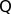
\includegraphics[scale=0.8]{figure/beispiel Netzwerk.png}
    \caption{Sample RC- network}
    \label{fig:sampleRCnetwork}
    \end{figure}
    The heat flux $\dot{Q}$, for example from a radiator, influences the temperature $T_{wall}$, as well as the capacitance $C$. And the temperature $T_{wall}$ affects the temperature inside and outside $T_{inside}$ and $T_{outside}$ with their resistances $R_{\alpha,inside}$ and $R_{\alpha,outside}$. The example shows that all connections in the network influence each other.
    To model the dynamics of the wall in differential equations, Kirchhoff's Current Law is required. It states that the sum of the flowing current to the node is equal to the sum of the flowing current of the node 
    \cite{Kuchling.2007}. 
    Because of the thermal analogy of electrical laws, the current is replaced by heat flux. The following differential equation results for the node  $T_{wall}$ using Ohm's law ($\dot{Q}=\Delta T/R$) and the relationship $\dot{Q}=C\frac{\partial T}{\partial t}$.     
    \begin{equation}
    \label{eq:sampledifferential}
    C \frac{\partial T_{wall}}{\partial t} = \dot{Q} + \frac{T_{inside}-T{wall}}{R_{\alpha,inside}} - \frac{T_{wall}-T{outside}}{R_{\alpha,outside}}
    \end{equation}
    In \autoref{fig:sampleRCnetwork}, the thermal resistances are serially connected. According to the electrical network, resistances in series are equal to their sum. 
    \begin{equation}
    \label{eq:resistanceseriel}
        R_{sum} = R_{\alpha,inside} + R_{\alpha,outside}
    \end{equation}
    A parallel circuitry has windows and walls in buildings, for example. Here the resistances are calculated according to the following schema:
    \begin{equation}
    \label{eq:resistancesparallel}
        \frac{1}{R_{sum}} = \frac{1}{R_{wall}} + \frac{1}{R_{window}}
    \end{equation}
    In terms of needed more capacitances for describing the thermal model, the summary capacitance is added in a parallel circuitry as: 
    \begin{equation}
    \label{eq:capacityparallel}
         C_{sum} = C_1 + C_2
    \end{equation}
    The serial circuitry of capacitances is calculated as follows:
    \begin{equation}
    \label{eq:capacityseriell}
         \frac{1}{C_{sum}} = \frac{1}{C_1} + \frac{1}{C_2}
    \end{equation}
    
%maschenregel noch erklären?


\section{Model predictive control (MPC)}
\label{section:mpc}

"The idea of model predictive control [...] is [...] to utilize a model of the process in order to predict and optimize the future system behavior"
\cite{Grune.2017}.
Applied to a thermal control of a building with the aim of grid-supporting, a model of the thermal behaviour of the building is required to predict the reaction of the system behaviour in the next $N$ time steps, called the prediction horizon. Every time step $k$, the current state $\mathbf{x_k}$, the output $\mathbf{y_k}$ is measured, and the future system behaviour is obtained computation. The computation of the future system behaviour may include weather forecast, occupancy schedule and the optimization of the control signal $\mathbf{u_k}$ over the optimization horizon $\mathbf{u_{k+N}}$. But, only the first calculated control signal is adopted as input for the plant.
Then, the calculations are repeated at every time step. \autoref{fig:sampleMPC} visualises the MPC control loop.
 \begin{figure}[h]
    \centering
    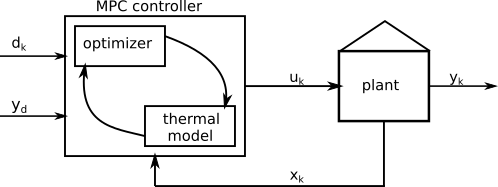
\includegraphics[scale=0.8]{figure/MPC beispiel2.png}
    \caption{MPC structure of the control loop}
    \label{fig:sampleMPC}
    \end{figure}
\newline
Concluded, the MPC is "an iterative online optimization over the predictions"
\cite{Grune.2017} 
compiled by the thermal model of the building. Mathematically explained, the optimizer needs to reduce the following equation according to
\cite{Kouvaritakis.2018}
and
\cite{Oldewurtel.2012}:
\begin{align}
\label{eq:costfunc}
\textrm{Cost function} && minimize \sum_{k=1}^{N-1} c_k(x_k,u_k,y_k)
\end{align}
subject to 
\begin{align*}
\textrm{Current state} && x_0 &=& x \\	
\textrm{Dynamics} && x_{k+1}&=& f(x_k,u_k,d_k)		&&	y_k = g(x_k,u_k,d_k)\\				
\textrm{Constraints} && y_{min}&\leq& y_k \leq y_{max}\\		
\textrm{} && u_{min}&\leq& u_k \leq u_{max}	
\end{align*}
$c_k$ represents the cost function, which is explained in detail in \autoref{subsection:costfunction}
. In terms of building control, $y$ is the internal temperature.
%Störungen noch erklären

\subsection{Cost function}
\label{subsection:costfunction}

    The cost function $c_k$ assigns a cost to the control signal $u_k$ and the current state $x_k$, which is mathematically described in
    \autoref{eq:costfunc}
    , with:
    \begin{equation}
    \label{eq:c_k}
    c_k = (x_k^TQx_k+u_k^TRu_k)
    \end{equation}
    Here $Q$ and $R$ are matrices over which individual elements of the state vector or control signal vector can be weighted differently.  
    \cite{Kouvaritakis.2016}
    %linear, quadratisch, gewichtet 
    %reduziert Zustand, stellsignal

\subsection{Current state}
\label{subsection:currentstate}

    The current state $\mathbf{x_k}$ is a vector of measured state variables of a building. Every prediction starts from this initial state \cite{Oldewurtel.2012}.
    
\subsection{Dynamics}
\label{subsection:dynamics}
    
    The state-space formulation (SSF) is an alternative representation of a linear differential equation, which models a physical system. In this work, it is used for the formulation of the thermal model, which is required for the MPC. The SSF consists of the state $\textbf{x}$, the control signal $\textbf{u}$, the disturbances $\textbf{d}$ and the output of the system $\textbf{y}$ represented in \autoref{eq:statespace}. The system matrix is $A$, $B_1$ and $B_2$ are called the input matrices, $C$ is the output matrix, $D_1$ and $D_2$ are the pass-through matrices.  
    \begin{align}
    \label{eq:statespace}
    \dot{\textbf{x}}=A\textbf{x}+B_1\textbf{u}+B_2\textbf{d}\\
    \textbf{y}=C\textbf{x}+D_1\textbf{u}+D_2\textbf{d} \notag
    \end{align}
    In a thermal model of a building, some authors (\cite{Hazyuk.2012}, \cite{Siroky.2011},...) use the state as a vector of some temperatures, the control signal as a signal for the heating system, the disturbances can describe the influence by the weather or occupants and the output of the system contains frequently the temperature inside of the building.
    


\subsection{Constraints}
\label{subsection:constraints}

Dealing with constraints is one of the most important advantages of MPC. Thereby, constraints can be used for the state, the output, and the input. In terms of building control, output constraints and input constraints are reasonable, as mathematically described in the \autoref{eq:costfunc}. That means, the output constraints could be a temperature range, which feels comfortable for occupants. And the constraints for the input are given as minimal (= 0) and maximal values of the possible performances. General, logical and physical ranges are constrained. There are different forms of constraints, but linear constraints are frequently used for MPC because they simplify the optimization problem. Constraints can also be time dependant. This is beneficial for embedding diverse temperature ranges during the night and the day or during the working time of occupants when they are not at home.
\cite{Siroky.2011}
%es gibt harte und weiche constraints. wichtig ist, dass man nicht auf beiden seiten harte constraints einstellt. konvexe Constraints bei bedarf

\chapter{Modelling}
\label{ch:modelling}
After explaining thermal basics and the electrical analogy, the foundations are used in this chapter. The creation of the thermal model of the reference building and the resulting thermal model are presented. Later, the model is needed for the MPC to predict the thermal reactions of the building.
\newline
    
    The focus of this work is on the MPC part, so a simple thermal model is required. Nevertheless, no necessary information must be missing. Therefore, the thermal storage possibilities, the temperature inside of the building, and the heating system's influence have to be represented in the model. The storage allows to heat during the grid has too much power and to save energy in the building during the grid requires power. Hence, this enables the MPC's objective of grid services. The output of the model needs to be the temperature inside since the MPC aims to be in a pleasant temperature range to ensure customer comfort. Last, the influence of the heating system must be recognisable in the model, as it is the input of the plant.
    \newline
    The thermal model records the thermal conditions of the reference building. Therefore, the inner energy of the water reservoir and the air temperature inside the building are modelled. The water reservoir and the building behaviour are modelled according to different modelling strategies. The following chapters describe the partial models water reservoir and building model, the kind of modelling, and the conclusion of the partial models.
    
    \section{The modelling strategies}
    \label{ModellingStrategies}
    Creating a model can be made with three types of models, the so-called white-box models, grey-box models or black-box models. White-box models describe the real system only physically. Black-box models, on the other hand, have no physical description. They are created with data. And grey-box models are in between these two options \cite{Statusseminar.ForschungfurEnergieoptimiertesBauen.2009}. All possibilities are used in the thermal modelling of buildings \cite{Kramer.2012}.
    \newline
    The chosen approach for the MPC is the \textbf{grey-box model} for two reasons: First, this approach combines the advantages of white-box models and black-box models \cite{EstradaFlores.2006}. Second, there is the possibility to generate the required data from the reference building with the available measurement equipment at KIT. According to Coakley et al., further advantages and disadvantages are among other things\cite{Coakley.2014}:
    \begin{table}[h!]
    \label{Advantages and disadvantages of grey-box modelling}
        \centering
        \begin{tabular}{p{7.3cm} | p{7.3cm}}
        \hline
          Advantages  &  Disadvantages\\
        \hline
        \begin{itemize}
            \item faster development by a combination of physical and statistical model
        \end{itemize}
      & \begin{itemize}
            \item requires knowledge in physical and statistical modelling 
        \end{itemize}\\
     \begin{itemize}
            \item accuracy of the results for the specific use case, provided by qualitative training data
        \end{itemize} & \begin{itemize}
            \item changes at the building lead to a re-training
        \end{itemize}\\
        \end{tabular}
        \caption {Advantages and disadvantages of grey-box modelling}
    \end{table}
    \newline
    However, the water reservoir and the heating system are not in use yet. So, no data are available for training a grey-box model. That's the reason why a part of the model needs to create as \textbf{white-box model}.
    \newline
    But also, white-box models have some pros and cons (see the following Table \cite{EstradaFlores.2006}).
    \begin{table}[]
    \label{tab:wihte-boxpro}
        \centering
        \begin{tabular}{p{7.3cm} | p{7.3cm}}
        \hline
          Advantages  &  Disadvantages\\
        \hline
        \begin{itemize}
            \item relies on physics
        \end{itemize}
      & \begin{itemize}
            \item needs assumptions to simplify 
        \end{itemize}\\
     \begin{itemize}
            \item applicable for every situation with the same assumptions and requirements 
        \end{itemize} & \begin{itemize}
            \item often complex mathematical problems
        \end{itemize}\\
        \end{tabular}
        \caption {Advantages and disadvantages of white-box modelling}
    \end{table}

    \section{The water reservoir model}
    \label{waterModel}
    First, all heat flows are regarded for modelling the water reservoir (WR), which influence the water reservoir (see \autoref{fig:Figure of the water reservoir with the heat flows}). The heat pump (HP) feeds the water reservoir with heat flow $\dot{Q}_\text{HP}$. The service water (SW) and the water for the heating circuit are taken from the storage. Since no service water is currently connected to the reference building, the heat flow $\dot{Q}_\text{SW}$ will be set to zero in the following. The heat losses $\dot{Q}_\text{loss}$ and the heating heat flow  $\dot{Q}_\text{heating}$ are consequently the discharged heat flows. The resulting energy balance according to \autoref{eq:1HS} follows below.
    \begin{equation}
        \label{waterReservoir}
        \frac{d U_\text{WR}}{d t}= -\dot{Q}_\text{heating} + \dot{Q}_\text{HP} - \dot{Q}_\text{loss}
    \end{equation}
    
    \begin{figure}
        \centering
        \def\svgwidth{120pt}
        \input{figure/Wasserspeicher.pdf_tex}
        \caption{Figure of the water reservoir with the heat flows}
        \label{fig:Figure of the water reservoir with the heat flows}
    \end{figure}
    Since the model are referred to a real building, the size of the heat flows and the inner energy are limited according to the devices of the building. The heating heat flow moves in a range according to the calculations of the heating system \cite{Roth_Auslegung.2020} and can also have negative values when cooling is required (then according to the calculations of the cooling load \cite{SEFIngenieurgesellschaftMBH.2019}). The heat losses and the heat pump heat range are taken from the technical data \cite{Oskar}, \cite{TUM}.\newline
    Since the reference water reservoir is a stratified storage we determine the maximum inner energy in assumption of two heat layers. According to \autoref{eq:innerEnergy}, we need material parameters of water ($c_\text{v,w}$, $\rho_\text{w}$), the size of the water reservoir ($m = \rho_\text{w} V$), both is known, and a temperature difference, which we define for both layers. We assume that we heat up the storage from ambient temperature $T_\text{amb}$ around 20°C in both layers. Even with negative outside temperatures, the characteristic diagram of the heat pump provides the maximum inlet temperature of 55 °C, which should be the maximum temperature of the upper layer in the water reservoir $T_\text{max,1}$. The maximum temperature of the lower layer $T_\text{max,2}$ orients towards the inlet temperature of the underfloor heating and lies by 35 °C. After that, we calculate the sum of the inner energy as follows.
    \begin{equation}
        \label{eq:max.Energie}
        U = \rho_\text{w} c_\text{v,w} ((T_\text{max,1}-T_\text{amb})*\frac{V}{2} + (T_\text{max,2}-T_\text{amb})*\frac{V}{2}) 
    \end{equation}

    \section{The building model}
    \label{building model}
    First, a physical description of the thermal dynamics of the building must be created. To obtain the condition of a simple model, we model the building as a single zone, as often practised in the literature \cite{Park.2011}, \cite{Hazyuk.2012}. Single zone means that we sum all relevant values of the rooms, such as air temperature or wall temperature, by averaging to one value. 
    \newline
    We consider the air temperature, the temperature of the outer walls, the temperature of the inner walls and floors in the first floor, and the temperature of the floor in the model. In the following, these temperatures are called: inside temperature  $T_\text{inside}$, envelope temperature $T_\text{envelope}$, interior temperature $T_\text{interior}$, and floor temperature $T_\text{floor}$. 
    Using the state-space formulation (see \autoref{subsection:dynamics}), the temperatures are states in this model. According to the RC-analogy (see \autoref{electricalanalogy}), the model is built and nearly explained in the following for every state. \newline%
    
    \textbf{Inside temperature:}\newline
    One focus lies on the accuracy of the inside temperature since this temperature will be controlled in the later prepared MPC. Therefore, a more precise description of the dynamics is required (see the following equation). We consider the influence of the sun $\dot{Q}_\text{sun,inside}$, the heating system $\dot{Q}_\text{heating}$ and the other states in the way shown in the following equation. $\dot{Q}_\text{heating}$  links the water reservoir model and the building model because the heat flow is the same but leaves the water reservoir model and enters the building model. 
    \begin{align}
        \label{eq:1.state}
        C_\text{inside}*\frac{d T_\text{inside}}{d t} &=& \dot{Q}_\text{heating} + \dot{Q}_\text{sun,inside} - \frac{T_\text{inside}-T_\text{envelope}}{R_\text{inside}} - \frac{T_\text{inside}-T_\text{outside}}{R_\text{window}} \\
       & &-\frac{T_\text{inside}-T_\text{interior}}{R_\text{interior}}-\frac{T_\text{inside}-T_\text{floor}}{R_\text{floor}}\nonumber
    \end{align}
    The detailed explanation for the composition of the thermal resistance and capacitance is in \autoref{electricalanalogy}. In the following table, the special material and state dependant values are explained.
    \begin{table}[H]
        \centering
        \begin{tabular}{l p{13cm}}
            $C_\text{inside}$ & The thermal capacitance $C_\text{inside}$ is calculated with the mass of the air from all rooms and the capacity of the air (1006 $J/(kg K)$ \cite{Weigand.2016}). The mass can be determined with the volume of the rooms according to the construction plan \cite{Bauplan} and the air density (1.28 $kg/m^3$ \cite{Weigand.2016}).\\
            $R_\text{inside}$ & The thermal resistances $R_\text{inside}$ includes a convective part with the transfer coefficient $\alpha = 0.9 W/(m^2 K)$ special for air perpendicular to the wall in buildings with the assumption of one Kelvin temperature difference between the wall and air \cite{Schweizer-fnalpha}.\\
            $R_\text{window}$ & The window resistance $R_\text{window}$ is determined with the window area and the assumption of a heat transmission coefficient $u = 1 W/(m^2 K)$ \cite{ThorbenFrahm.2021}.\\
            $R_\text{floor}$ & Heat conductivity and heat convection are the regarded mechanisms to determine the floor resistance $R_\text{floor}$. The floor material is reinforced concrete with the thermal conductivity of $2.3 W/(m K)$ \cite{AntonSchweizer.12.10.2021}.\\
            $R_\text{inside}$ & For the convection in the inner of the building, the same assumptions are made as for $R_\text{inside}$.\\
            $R_\text{interior}$ & The interior resistance $R_\text{interior}$ is also calculated with the heat transfer coefficient inside.
        \end{tabular}
        \caption{Explanation of the special material and state dependant values of the differential equation of the inside temperature}
        \label{tab:valuesOfInsideTemperature}
    \end{table}
    
    \textbf{Envelope Temperature:}\newline
    The sun, the contact of the walls with the inner air temperature and with the outside temperature influence the envelope temperature. The sun affects the air temperature in another area ratio than the outer walls. Therefore, we difference the influence of the sun on the inner air temperature and the envelope, and we consider here $\dot{Q}_\text{sun,envelope}$.  
    \begin{equation}
    \label{eq:diffEnvelope}
        C_\text{envelope}*\frac{d T_\text{envelope}}{d t} = \dot{Q}_\text{sun,envelope} - \frac{T_\text{envelope}-T_\text{outside}}{R_\text{envelope}} + \frac{T_\text{inside}-T_\text{envelope}}{R_\text{inside}}
    \end{equation}
    \begin{table}[H]
        \centering
        \begin{tabular}{l p{13cm}}
        $R_\text{envelope}$ & The outer wall resistance $R_\text{envelope}$ contains a heat conductivity of aerated concrete ($0,133 W/(m K)$ \cite{GhaziWakili.2015}) and the heat transfer coefficient for air perpendicular to the wall outside $\alpha_\text{envelope}$ according to the rules of thumb from Schweizer-fn \cite{Schweizer-fnalpha}
    \begin{equation}
        \alpha_\text{envelope} = 3,96 (v / L)^0,5 = 1,669 W/(m^2 K)
    \end{equation}
    with the average wind velocity of Karlsruhe $v$ \cite{AbteilungKlimaundUmweltberatung.2004} and the length of the building wall.  \\
        $C_\text{envelope}$ & To determine the capacitance $C_\text{envelope}$, we need the volume of the outer walls from the construction plan \cite{Bauplan}, the density of aerated concrete ($485 kg/m^3$) and the capacity (1000 $J/(kg K)$) \cite{GhaziWakili.2015}. 
        \end{tabular}
        \caption{Explanation of the special material and state dependant values of the differential equation of the envelope temperature}
        \label{tab:valuesOfEnvelopeTemperature}
    \end{table}
   
    \textbf{Interior and floor temperature:}\newline
    The differential equations for the interior and the floor temperature are as simple as possible. Both states have just an impact on the inside temperature. 
    Hazyuk et al. models for example also the ground floor as one state \cite{Hazyuk.2012}. The explanation is that the ground floor has no convective contact with the environment. Therefore, he is not modelled with the envelope for holding the physical structure, where the wind has an impact on the outer walls.
    The interior is extra modelled to improve the accuracy of the inside temperature equations because the capacitance of the inner walls is specially collected.
    \begin{align}
    C_\text{interior} \frac{d T_\text{interior}}{d t} &= \frac{T_\text{inside}-T_\text{interior}}{R_\text{interior}} \\
       C_\text{floor} \frac{d T_\text{floor}}{d t} &= \frac{T_\text{inside}-T_\text{floor}}{R_\text{floor}} \nonumber\\
    \end{align}
    As above, we need some material parameters for the calculation of the capacitance $C_\text{floor}$ and $C_\text{interior}$. The material of the floor is reinforced concrete and the interior' material is aerated concrete. The previously unnamed material parameters are the density ($2500 kg/m^3$) \cite{AntonSchweizer.12.10.2021} and the capacity ($880 J/(kg K)$) \cite{AntonSchweizer.12.10.2021b} of reinforced concrete.\newline
     
    Summarising, \autoref{fig:structureThermalModel} illustrates the building model with all its connections according to the RC- analogy.
    \begin{figure}
            \centering
            \def\svgwidth{410pt}
            \input{figure/meinModel2.pdf_tex}
            \caption{Structure of the thermal model in RC- analogy}
            \label{fig:structureThermalModel}
        \end{figure}
        
    \subsection{Parameter identification}
    \label{WorkflowModel}
    
     \begin{figure}
            \centering
            \def\svgwidth{400pt}
            \input{figure/workflow greybox modelling.pdf_tex}
            \caption{Work flow of grey-box modelling with Matlab}
            \label{fig:workflowModel}
    \end{figure}
    \autoref{fig:workflowModel} explains the procedure, how to generate the grey-box model from the physical building model.\newline 
    The used toolbox from Matlab is the "System Identification Toolbox". For this application, the most important commands are "idgrey" and "greyest".
    With the idgrey-command, we can specify the building model as the initial model for the grey-box estimation in state-space formulation. That means the thermal resistances and capacitance, which we determined above, are the initial values for the estimation and they are the values, which the estimator from Matlab can vary. We add also the parameters $f_\text{sol,inside}$ and $f_\text{sol,envelope}$ for estimating because we model in the simplest way the heat flow of the sun isolation $\dot{Q}_\text{sun,envelope}$ and $\dot{Q}_\text{sun,inside}$ with the measured diffuse insolation $I_\text{sun}$ (see the following equation). 
    \begin{align}
       \label{eq:sun}
        \dot{Q}_\text{sun,inside} &= f_\text{sol,inside} I_\text{sun} \\
        \dot{Q}_\text{sun,envelope} &= f_\text{sol,envelope} I_\text{sun} \nonumber 
    \end{align}
    The initial values for $f_\text{sol,inside}$ and $f_\text{sol,envelope}$ are chosen as $0.25$ according to Harb et al. \cite{Harb.2016}. And, we replace in the differential equation of the envelope temperature from \autoref{eq:diffEnvelope} the thermal resistance $R_\text{inside}$ to $R_\text{in}$. The initial values of $R_\text{inside}$ and $R_\text{in}$ are the same, but we obtain more flexibility in the grey-box model, if we estimate both values.\newline
    After that, we look for the data from the reference building. The data are generated in an experiment, but this is explained in a subsequent chapter. When we have the data, they are separated into training data and verification data. The training data are used for the estimation. From the reference building, we obtain the room temperatures, which we average with the capacitance of each room to one value, the inside temperature. The same procedure is adopted for the outer wall temperature, except that the outer wall temperatures are averaged with their own capacitance. The interior and the floor temperatures are determined in the same way. Also, we obtain data of the heating system for $\dot{Q}_\text{heating}$ and the weather specially the outside temperature $T_\text{outside}$ and the diffuse insolation $I_\text{sun}$ for determining $\dot{Q}_\text{sun,envelope}$ or $\dot{Q}_\text{sun,inside}$. \newline
    Now, the greyest-command executes the parameter identification with the training data. The used search method of the greyest-command is subspace Gauss-Newton least squares search. The table below summarizes the modelling parameters for the estimation. The states $T_\text{inside}$ and $T_\text{envelope}$ are also defined as the output to be optimized. For the later MPC, $T_\text{inside}$ is the only relevant output. However, we expect better results for the whole model during optimizing the two states with the more complex differential equations. 
    At last, we obtain the ready model (see in \autoref{sec:appendix:Modelvalues} the initial values and the identified values).
     
    \begin{table}[]
        \centering
        \begin{tabular}{p{5cm}|p{8cm}}
        Parameters to be identified &  $C_\text{inside}$,  $C_\text{envelope}$,  $C_\text{interior}$, $C_\text{floor}$, $R_\text{inside}$, $R_\text{window}$, $R_\text{envelope}$, $R_\text{interior}$, $R_\text{floor}$, $R_\text{in}$, $f_\text{sol,inside}$, $f_\text{sol,envelope}$ \\
        &\\
        Inputs & $\dot{Q}_\text{heating}, I_\text{sun}, T_\text{outside}$\\
        &\\
        Outputs to be optimized & $T_\text{inside}, T_\text{envelope}$
        \end{tabular}
        \caption{Conclusion of relevant information about the grey-box model}
        \label{tab:Greybox}
    \end{table}
    
    \subsection{Training and verification of the thermal model}
    \label{verificationthermalmodel}
    The training data set comprise twelve days from 23 July to 4 August 2021, including a heating period from 26 July to 1 August 2021. The verification data set is half the size of the training data set (from 13 July to 19 July 2021), also including a heating period from 16 July to 18 July 2021. \newline
    \begin{figure}
            \centering
            %\def\svgwidth{100pt}
            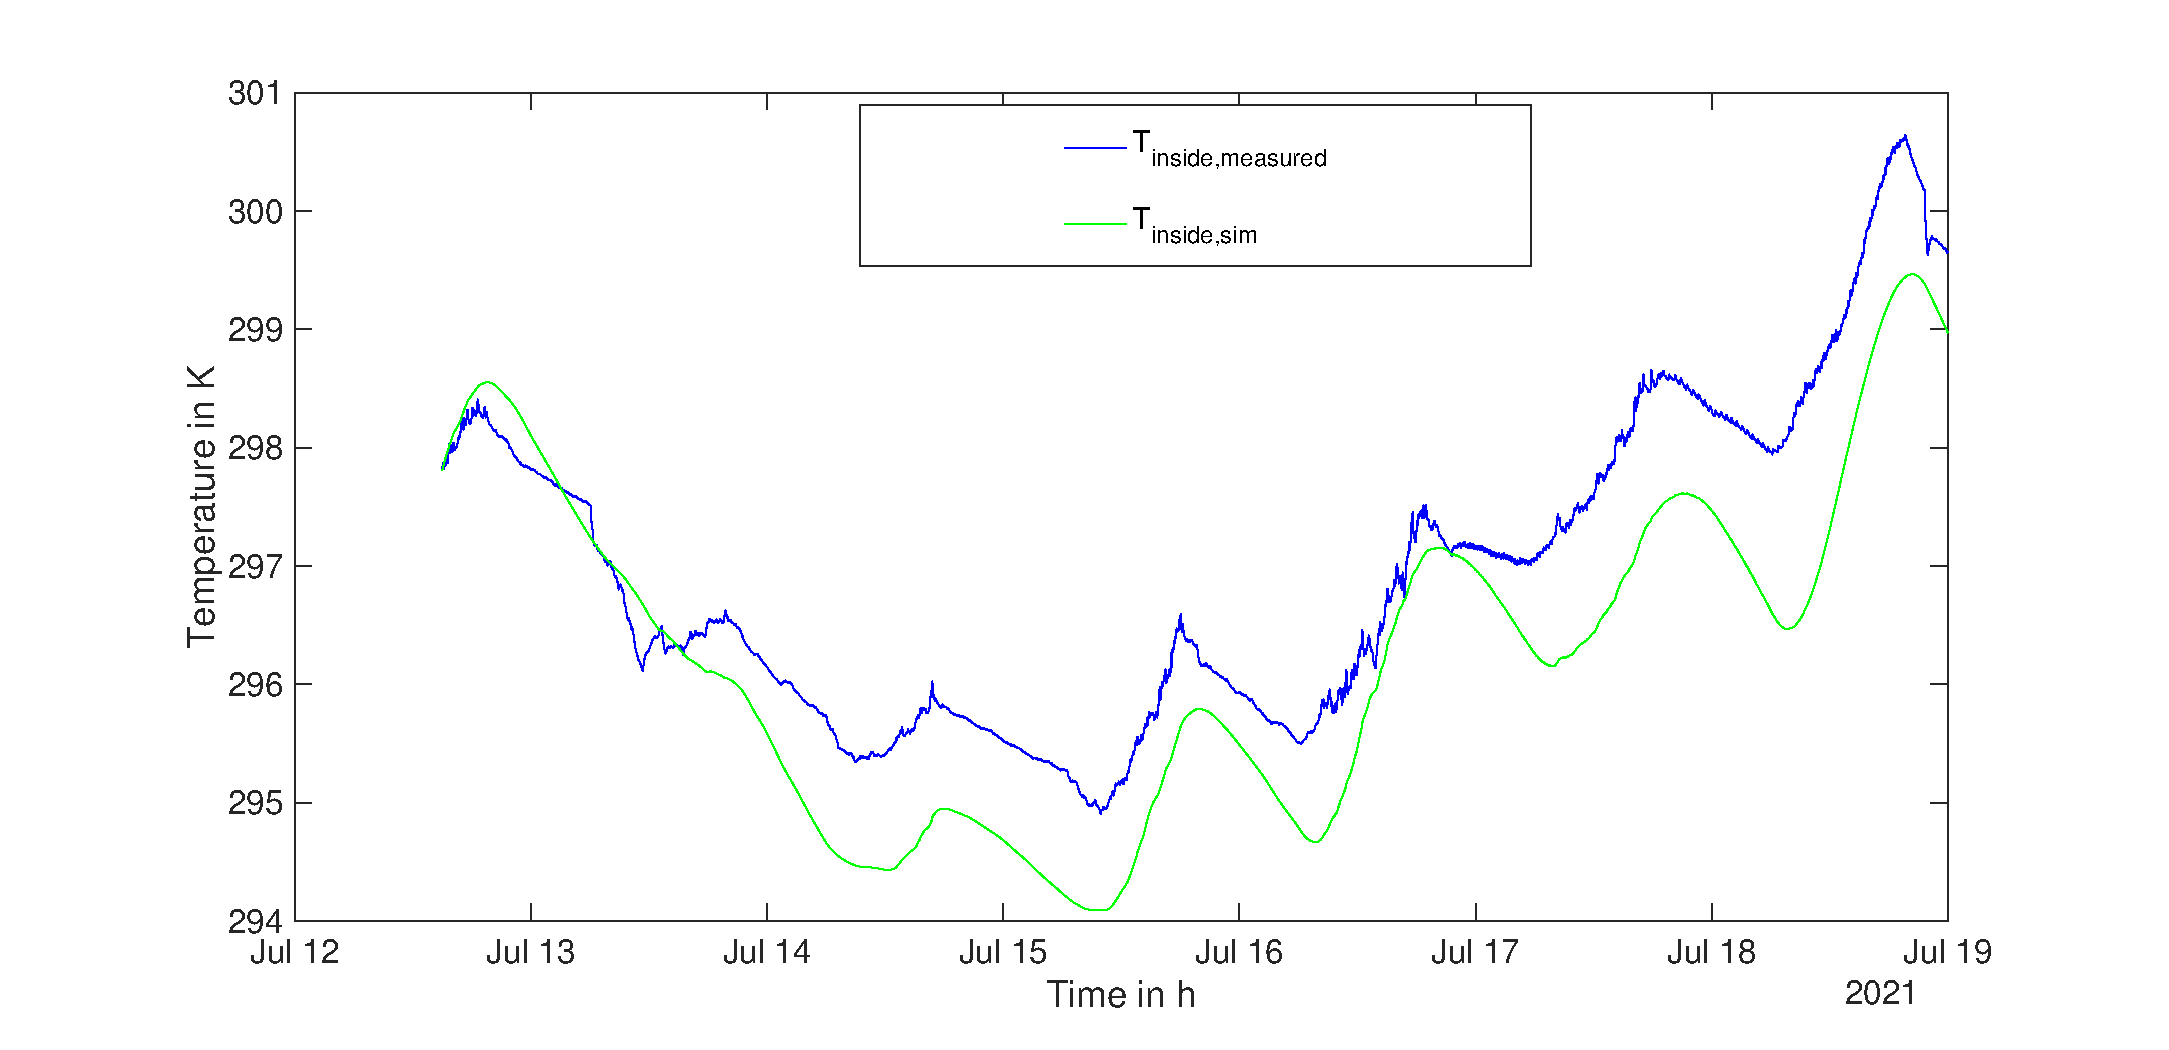
\includegraphics[width=7cm,height=5cm]{figure/Verlauf_inside_ValidierungModell.eps}
           \caption{Verification of the building model}
           \label{fig:verificationModel}
    \end{figure}
   \autoref{fig:verificationModel} shows the curve of the inside temperature of the simulated and the measured values. It is noticeable that the model reflects the dynamic of reality sufficiently. In addition, the Root Mean Square Error (RMSE) and the maximum residual ($\mathrm{R}_\text{max}$) is used as verification measure of the model.\newline
    The RMSE is calculated with the quadratic difference of the simulated output $y_\text{sim}$ and the measured output $y_\text {meas}$ as follows \cite{Barnston.1992}: 
    \begin{equation}
        RMSE = \sqrt{\frac{1}{N} \sum \limits_1^N (y_\text{sim} - y_\text {meas})^2}
    \end{equation}
    Here is $N$ the number of measurements or simulated values.
    Based on the \autoref{tab:RMSEundR} presented RSME and $\mathrm{R}_\text{max}$, it can be shown that during the training and verification period, the magnitudes of the RSME and $\mathrm{R}_\text{max}$ are similar. The results of the RMSE and the $\mathrm{R}_\text{max}$ are listed for the two optimized outputs after the training and the verification period.
     \begin{figure}[h]
    \begin{minipage}[t]{0.5\textwidth}
    \vspace{0pt}
        \begin{tabular}{c|c|c|c|c}
             & \multicolumn{2}{|c}{$T_\text{inside}$} & \multicolumn{2}{|c}{$T_\text{envelope}$} \\
             \hline
            RMSE & \cellcolor{gray} 0.61 K & \cellcolor{gray90} 0.59 K & \cellcolor{gray} 0.49 K & \cellcolor{gray90} 0.52 K \\
            $\mathrm{R}_\text{max}$ &\cellcolor{gray} 1.45 K & \cellcolor{gray90} 1.62 K & \cellcolor{gray} 1.22 K & \cellcolor{gray90} 1.03 K
        \end{tabular}
    \end{minipage}
    \hfill
    \begin{minipage}[t]{0.5\textwidth}
    \vspace{0pt}
        \begin{tabular}{c c}
        \\
            &\cellcolor{gray} Training period \\
           &\cellcolor{gray90} Verification period
        \end{tabular}
    \end{minipage}
    \caption{RMSE and $\mathrm{R}_\text{max}$ of the output for training and verification period}
    \label{tab:RMSEundR}
    \end{figure}
    The maximum difference between the training and verification period for the RMSE lies by 0.3 K and for the $\mathrm{R}_\text{max}$ by 0.19 K. As a result, we can verify the building model.  

    \section{The state-space formulation}
    \label{holeModel}
    The white-box model of the water reservoir and the grey-box model of the building behaviour have now been prepared. In the next step, we put them together in the state-space formulation, which we introduced in \autoref{subsection:dynamics}, just as the MPC requires.\newline
    The separation in control signal $\textbf{u}$ and disturbances $\textbf{d}$ is important for this. The control signals are the heat flow of the heating system and the heat pump in the reference building. The main disturbances are the weather and, especially for the water reservoir, heat losses. Therefore, the state-space formulation looks as follows: 
  \begin{align}
	    \label{eq:ZRD Modell}
	 \left(\begin{array}{c} \frac{d T_{inside}}{d t} \\ \frac{d T_{envelope}}{d t} \\ \frac{d T_{interior}}{d t}\\ \frac{d T_{floor}}{d t}\\ \frac{d U_{WR}}{d t} \end{array}\right) &= A \left(\begin{array}{c} T_{inside} \\ T_{envelope} \\ T_{interior}\\ T_{floor}\\ U_{WR} \end{array}\right) + B_\text{1} \left(\begin{array}{c} \dot{Q}_{heating} \\ \dot{Q}_{HP} \end{array}\right) + B_\text{2} \left(\begin{array}{c} I_{sun,inside}\\ I_{sun,envelope}\\ T_{outside} \\ \dot{Q}_{loss} \end{array}\right) \\
	 T_{inside} &= C \left(\begin{array}{c} T_{inside} \\ T_{envelope} \\ T_{interior}\\ T_{floor}\\ U_{WR} \end{array}\right) \nonumber
	\end{align}	
    The hole matrices $A$, $B_\text{1}$, $B_\text{2}$, and $C$ are in \autoref{sec:appendix:Matrizen}. We have no pass-through matrices because neither control signals nor disturbances have a direct impact on the output. 
     
    
    






%\begin{align}
  %% C_\text{inside}*\frac{d T_\text{inside}}{d t} &=& \dot{Q}_\text{heating} + \dot{Q}_\text{sun,inside} - \frac{T_\text{inside}-T_\text{envelope}}{R_\text{inside}} - \frac{T_\text{inside}-T_\text{outside}}{R_\text{window}} \\
       %& &-\frac{T_\text{inside}-T_\text{interior}}{R_\text{interior}}-\frac{T_\text{inside}-T_\text{floor}}{R_\text{floor}} \nonumber\\
      % C_\text{envelope}*\frac{d T_\text{envelope}}{d t} &=& \dot{Q}_\text{sun,envelope} - \frac{T_\text{envelope}-T_\text{outside}}{R_\text{envelope}} + \frac{T_\text{inside}-T_\text{envelope}}{R_\text{inside}} \nonumber \\
     %  C_\text{interior}*\frac{d T_\text{interior}}{d t} &=& \frac{T_\text{inside}-T_\text{interior}}{R_\text{interior}} \nonumber\\
    %   C_\text{floor}*\frac{d T_\text{floor}}{d t} &=& \frac{T_\text{inside}-T_\text{floor}}{R_\text{floor}} \nonumber\\
    %   \frac{d U_\text{WR}}{d t}&=& -\dot{Q}_\text{heating} + \dot{Q}_\text{HP} - \dot{Q}_\text{loss} - \dot{Q}_\text{SW} \nonumber
  %  \end{align}
\chapter{Model predictive control}
\label{ch:mpc}
In this chapter, the framework conditions of the MPC are described by answering the questions: (i) what is controlled? (ii) How is controlled? (iii) Which curves are controlled? (iii) What data are used? Also, the constraints, the cost function, and the workflow of the MPC script are introduced. The objective of this investigation is to obtain a control signal for the heat pump of the reference building that considers grid services and occupancy comfort. There, the investigation stays in a simulation environment. \newline

\section{Framework conditions of the MPC}
\label{section:FrameworkMPC}
The objective of the MPC is to optimise the control signal of the reference building $\mathbf{u} = (u_1 \enspace u_2)^T = (\dot{Q}_\text{heating} \enspace \dot{Q}_\text{HP})^T$. Thereby, we consider the heat flows of the building in the MPC simulation but, we calculate with a characteristic diagram of the heat pump the electrical control signal $P_\text{HP}$ later. The controlled output is the inside temperature $\mathbf{y} = T_\text{inside}$, which we calculate with the thermal model from \autoref{holeModel}. The desired curves of the $\mathbf{y}$ depend on the presents of occupants, which is determined on an occupancy schedule. Past data of the weather and the dynamic price of the electricity $dP$ \nomenclature[P]{dP}{dynamic Price of the electricity } is used for the simulation environment. 

\subsection{Characteristic diagram of the heat pump}
\label{subsec:charcteristicDiagramHP}
The characteristic diagram of the heat pump is interpolated with the characteristic values specified by the producer \cite{TUM}. We assume an operation at the nominal power of the heat pump. As \autoref{fig:HeatpumpKennfeld} shows, the electrical power $P_\text{HP}$ depends on the outside temperature $T_\text{outside}$ and the required heat flow $\dot{Q}_\text{HP}$. Further, the heat pump can generate negative $\dot{Q}_\text{HP}$ when cooling is desired. The optimisation of the MPC computed the $\dot{Q}_\text{HP}$, and the $T_\text{outside}$ is known at every time step, then the characteristics of the heat pump are used to calculate the $P_\text{HP}$. 
    \begin{figure}[h]
            \centering
            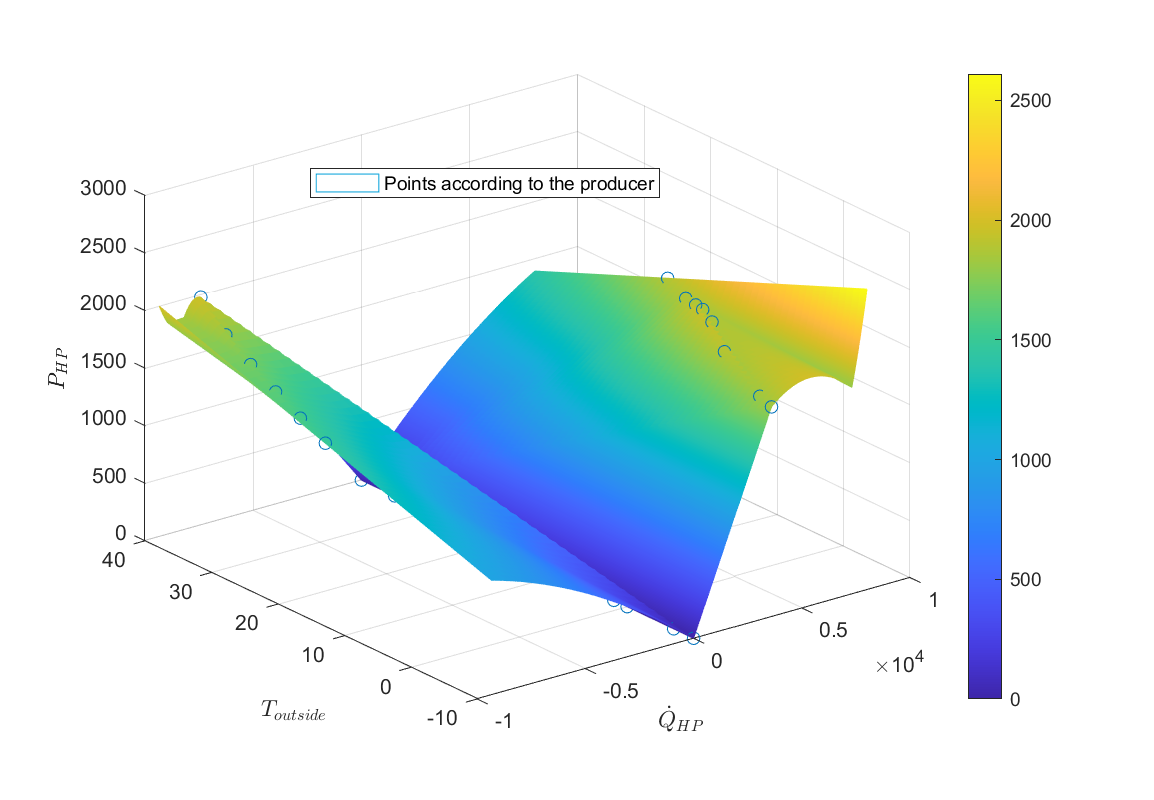
\includegraphics[width=8cm,height=6.5cm]{figure/HeatPumpV55nenn.eps}
           \caption{Interpolation of the characteristic diagram of the heat pump with nominal power according to \cite{TUM}}
           \label{fig:HeatpumpKennfeld}
    \end{figure}
    
\subsection{Occupancy schedule}
\label{subsec:OccupancySchedule}
The \autoref{fig:OccupancySchedule} presents the occupancy schedule. It summarises the working time of occupants with a green bar. We assume that persons are in the reference building from Monday to Thursday from 6 am to 7 pm and on Friday from 6 to 6 pm. The assumption is made according to experience values and means that there is a high probability that persons will be in the building during this time.  
    \begin{figure}[h]
            \centering
            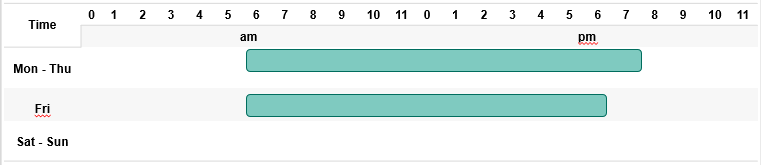
\includegraphics[width=15cm]{figure/Occupancy schedule.PNG}
           \caption{Occupancy schedule of the reference building}
           \label{fig:OccupancySchedule}
    \end{figure}

\subsection{Past data}
\label{subsec:PastData}
    The data used are from the same period as the training data for the model estimation. As a disturbance variable, we use the recording of diffuse radiation and outside temperature in Energy Lab 2.0. The MPC is simulated over nine days, a little more than a week, to consider the occupancy schedule at least  once.\newline
    The dynamic price of the electricity  $dP$ is made available on the website of the Bundesnetzagentur \cite{Bundesnetzagentur-smard}. Here we use the wholesale prices on the stock exchange as an indicator of grid services. The price is an intersection between supply and demand. Consequently, when the price is low, we can assume an excess of electricity on the grid. It is precisely then that it is particularly suitable to operate our heat pump to obtain electricity from the grid. In the opposite case, the same applies: If the price is high, it is unfavourable to operate the heat pump. At such a time, it is particularly suitable to supply power from the grid. In the opposite case, the same applies: if the price is high, it is unfavourable to operate the heat pump. \newline
    However, negative prices can also arise in retail. Negative prices would undesirably change the costs of the cost function, which will be explained in more detail later at a suitable time. To avoid negative prices, we sum the absolute minimum value of the $dP$ to every value of $dP$. Thus, we shift the curve of $dP$ into positive, as shown in \autoref{fig:Gridverschiebung}.
    \begin{figure}[h]
            \centering
            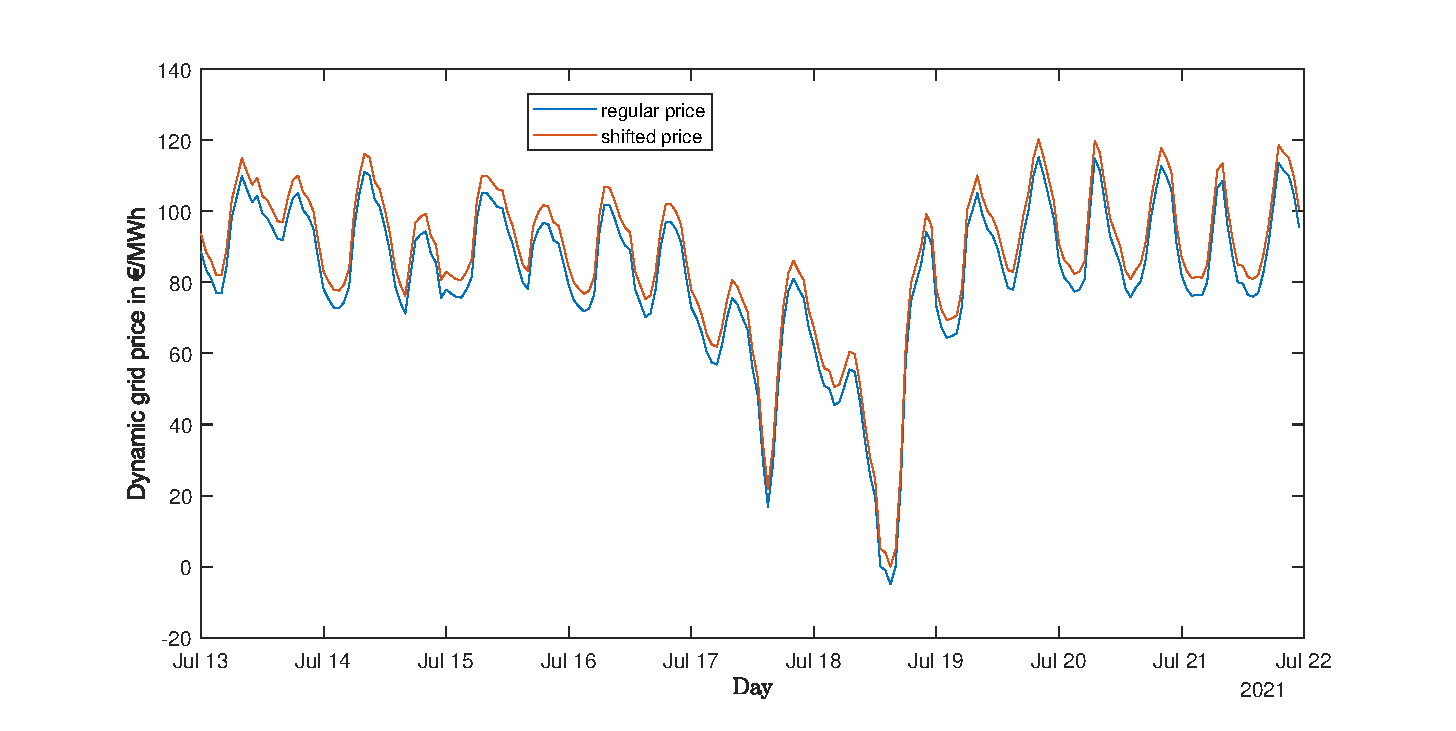
\includegraphics[width=15cm,height=8cm]{figure/Grid_data_Verschiebung.eps}
           \caption{Dynamic price of electricity \cite{Bundesnetzagentur-smard} and shifted dynamic price of electricity}
            \label{fig:Gridverschiebung}
    \end{figure}
    
\section{The Constraints}
\label{section:theconstraints}

The constraints depend on the physical limitations of the installations in the building, such as the heat pump, the underground floor heating, and the water reservoir, or of comfortable reasons. Also, the integration method of the model is included in the constraints. The subsequent section gives an overview of the constraints.

\subsection{Constraints of the control signals}
\label{subsec:COnstraintU}
The producer's specifications restrict $\dot{Q}_\text{HP}$ the maximum and minimum heat flow of the heat pump for nominal power by heating with the inlet temperature of 55°C and by cooling with the inlet temperature of 18°C \cite{TUM}. The maximum $\dot{Q}_\text{heating}$  is limited according to the underground floor heating calculation, where the set power of every room is counted and we sum it for the complete building \cite{Roth_Auslegung.2020}. The computation of the required cooling power predicts 2246 W needed power by 34.5°C outside temperature in July \cite{SEFIngenieurgesellschaftMBH.2019}. To be more flexible with higher outside temperatures, we round the minimum $\dot{Q}_\text{heating}$ to 2300 W.\newline
Further, we define a constraint $u_1 \cdot u_2 \geq 0$ to avoid simultaneous heating of building and cooling of the water reservoir or reversed. That would be energy waste.
The set $\mathbb{U_k}$ summarise mathematically the constraints.
\begin{equation}
    \label{ConstraintU}
    \mathbb{U_k} = \{\mathbf{u_k}| -2300 W \prec \dot{Q}_\text{heating} \prec 5283 W \wedge -9340 W \prec \dot{Q}_\text{HP} \prec 8010 W | u_1 \cdot u_2 \geq 0\} 
\end{equation}

\subsection{Constraint of output}
\label{subsec:constrainY}
The Umweltbundesamt \cite{Umweltbundesamt.7.10.2021} recommends an inside temperature of 18°C for some rooms, such as the kitchen. We expand the recommendation to a minimum $T_\text{inside}$ of 18°C for all rooms. The maximum inside temperature refers to the German technical rules for workplaces \cite{Bund.2021}, wherein a maximum of 26°C as room temperature is prescribed. The slack variable $\eta_\text{k}$ allows a variance of the given temperature range during a penalty in the cost function. Thus, we have a soft constraint, and we can obtain the feasibility of the optimisation problem during a deviation of the temperature range \cite{Drgona.2020}. The constraint is represented in the set $\mathbb{Y_k}$ as follows:  
\begin{equation}
    \label{ConstraintY}
    \mathbb{Y_k} = \{\mathbf{y_k}| 18 \text{°C} - \eta_k \prec T_\text{inside} \prec 26 \text{°C}+ \eta_k\} 
\end{equation}

\subsection{Constraints of the states}
\label{ConstraintX}
The calculation of the water reservoirs maximal inner energy $U_\text{WR}$ is explained in \autoref{waterModel} with \autoref{eq:max.Energie}. The minimum $U_\text{WR}$ lies by 0 J. The set $\mathbb{X}_{5,k}$ describes the constraint for the fifth element of the state vector.
\begin{equation}
    \label{ConstraintX5}
    \mathbb{X}_{5,k} = \{x_\text{5,k}| 0 J \prec U_\text{WR} \prec 96370000 J\} 
\end{equation}
A further constraint, which relates to the states, is the integration method as discussed below.

\subsection{Integration method and its constraint}
\label{COnstaintIntegration}
As an integration method, we use a explicit single-step method,which means that we need the values of the actual time step $k$ to compute the next. Possible methods are the Heun's method, the Euler and the Runge-Kutta method. The decision is made in favor of the Runge-Kutta method because the fourth order makes it more precise than the methods mentioned. The following equation shows the calculation for the next time step using the Runge-Kutta method with the sample time $T_\text{s}$ and the function $f(\mathbf{x_k},t_\text{k},\mathbf{u_k},\mathbf{d_k}) = \mathbf{\dot{x}_\text{k}}$ according the state-space formulation (see \autoref{eq:statespace}) \cite{KaiFurmansMarcusGeimerBalazsPritzCarstenProppe.WS1920}.

    \begin{align}
        \label{Runke-Kutta}
        a_k^{(1)} = T_s \cdot f(\mathbf{x_k},t_\text{k},\mathbf{u_k},\mathbf{d_k}) \\
        a_k^{(2)} = T_s \cdot f(\mathbf{x_k}+\frac{a_k^{(1)}}{2},t_k+\frac{T_s}{2},\mathbf{u_k},\mathbf{d_k})\nonumber\\
        a_k^{(3)} = T_s \cdot f(\mathbf{x_k}+\frac{a_k^{(2)}}{2},t_k+\frac{T_s}{2},\mathbf{u_k},\mathbf{d_k})\nonumber\\
        a_k^{(4)} = T_s \cdot f(\mathbf{x_k}+a_k^{(3)},t_k+T_s,\mathbf{u_k},\mathbf{d_k})\nonumber\\
        \nonumber\\
        \mathbf{x_{k+1}} = \mathbf{x_k} + \frac{1}{6}\cdot (a_k^{(1)} + 2 a_k^{(2)} + 2 a_k^{(3)} + a_k^{(4)})\nonumber
    \end{align}
    
Das Integrationsverfahren wird in den Constraints eingebunden, damit der folgenden Zeitschritt nach dem thermischen Modell berechnet wird.  
Wichtig zu beachten ist, dass die Schrittweiten der integration entsprechend der diskretisierung des models gewählt wird. So wird das Model mit mit diskreten werten aus dem reference gebäude geschätzt, wobei die Messstellen alle zwei Minuten abgetastet werden. Um beispielsweise eine Ts von einer Stunde zu erhalten, wird die Ts als 30 *2 min beschrieben. Die zwei minuten sind durch die schätzung bereits im modell enthalten, wir müssen das $\mathbf{\dot{x}_\text{k}}$ folglich nur mit 30 multiplizieren um einen Zeitschritt von einer Stunde weiterzukommen. Es ist wichtig zu beachten, dass das thermische modell aus zwei untermodellen zusammengesetzt ist. Das untermodell water reservoir, welches nach dem white-box ansatz modelliert wurde, benötigt eine andere Umrechnung um einen Zeitschritt von einer Stunde vorran zu gehen. Hier rechnen wir W in J pro Stunde um. In der MPC wirde dieser Unterschied direkt in der State-space formulation des modells durch einen faktor ausgeglichen.

\section{The Cost function}
\label{section:thecostfunction}

The cost function penalise the deviation from the desired requirements. On the one hand, we have to guaranty thermal occupant comfort in the building. On the other hand, we prefer to heat with the heat pump during convenient grid service. Both subjects are represented in the cost function below.
    \begin{equation}
        \text{minimize} \sum_{k=1}^{N-1} w_\text{1}\cdot (y-y_\text{track})^2 + w_\textbf{2}\cdot(u_\text{2}\cdot dP)^2 + w_\text{3} \cdot \eta^2
    \end{equation}
A pleasant air temperature is 22°C in rooms following the operative temperature in \cite{}. Therefore, the desired temperature is $y_track = 22$°C.
    %Erklären warum netzkurve verschoben werden musste: positive/neagtives Stellsignal und pos/neg Preis --> Auswrikungen durch quartrierung
    
    %hier erklären, wann gewicht = 0 flexibilität und energy sparen ist und Faktor 1/4 erklären
\section{Workflow of the MPC script}
\label{section:workflowMPC}
\begin{figure}[h]
            \centering
            \def\svgwidth{0.6\textwidth}
            \input{figure/workflowMPC.pdf_tex}
            \caption{Workflow of the MPC script}
            \label{fig:workflowMPC}
    \end{figure}
    
\section{Choice of weightings and horizon}
\label{Choise of weigtings and horizon}
\chapter{Results}
\label{ch:results}
In this chapter, different scenarios are considered to answer the research question focusing on grid services. Several scenarios are supposed to explain how the occupancy schedule affects energy consumption, grid service and comfort: (i) a scenario with an occupancy schedule, in which the MPC has to comply with fewer restrictions during the absence of occupants; (ii) a scenario that also has a lower temperature specification during the absence; and (iii) a scenario without an occupancy schedule. In the last section, the results are evaluated, and an answer to the research question is found.

\section{Results of the scenarios}
\label{sec:ResultsScenarios}
In this section, the implementation of the different scenarios is explained and the results of the temperature and control signal curves are presented. Furthermore, energy consumption, comfort and grid services are evaluated.  

\subsection{Presentation of the scenarios}
\label{subsec:Presentation of the scenarios}

\textbf{(i) The basic scenario:}\newline
The first considered scenario is the basic scenario, which is explained in detail in \autoref{ch:mpc}. Summarised, we desire the $T_\text{inside}$ during the presence of occupants as 22°C. And we leave the optimiser free to find an optimal temperature in the specified temperature range during the absence realised by neglecting the comfort requirement in the cost function.\newline

\textbf{(ii) Scenario 2:}\newline
The Umweltbundesamt \cite{Umweltbundesamt.7.10.2021} recommends during the absence of persons a room temperature of 17°C. Therefore, we consider scenario 2 with the desired $T_\text{inside}$ during the presence of occupants with 22°C and during absence with 17°C. In the opposite to the basic scenario, we do not change the cost function \ref{eq:costfunctatsächlich} during presence and absence but the $y_\text{track}$. Using one more symbolic parameter in the optimisation, which is set by the occupancy schedule to $y_\text{track,day}$ or $y_\text{track,night}$ we achieve the implementation of scenario 2. In addition, the temperature range needs to enlarge because the lower bound requires to be under the requested temperature. Thus, we choose 16.5°C as a lower bound. The set of constraints changes to:
\begin{equation}
    \label{ConstraintYScenario2}
    \mathbb{Y_k} = \{\mathbf{y_k}| 16.5 \text{°C} - \eta_k \prec T_\text{inside} \prec 26 \text{°C}+ \eta_k\} 
\end{equation}
The MPC algorithm has to handle significant fluctuations of the desired temperature. Therefore we reduce the weighting $w_\text{3}$ to minimum needed depending on the $w_\text{1}$ and $w_\text{2}$. In this way, we allow more deviations of the desired temperature to obtain a feasible solution of the MPC. \newline 

\textbf{(iii) Scenario 3:}\newline
Scenario 3 is for the optimisation problem the simplest one. The desired $T_\text{inside}$ is the 22°C over the complete simulation time. This case does also not consider the occupancy schedule. We can use the cost function \ref{eq:costfunctatsächlich} without changes during the time.

\subsection{Results of the scenarios}
\label{subsec:Results of the scenarios}
    \begin{figure}[h]
            %\centering
            \def\svgwidth{1.3\textwidth}
            \input{figure/HP_grid2.pdf_tex}
            \caption{}
            \label{fig:HP_grid}
    \end{figure}
%Verlauf temperatur und Stellgrößen, Angabe zu Energieverbrauch, Komfort und Grid services + nach verschiedenen Gewichten
\section{Discussion}
\label{sec:discussion}

\subsection{Comparison of the scenarios}
\label{subsec:Comparison fo the scenarios}

 % Nur wegen Netzdienlichkeit Scenario 2 überhaupt interessant. 
\subsection{General discussion about the approach}
\label{subsec:General discussion about the approach}

%This chapter is supposed to discuss your results. Point out what your results mean.
%What are the limitations of your approach, managerial implications or future impact?
%
%Explain the broader picture but be critical with your methods.
\chapter{Conclusion and outlook}
\label{ch:Conclusionandoutlook}

\section{Conclusion}
\label{sec:conclusion}
Increasing fluctuations due to more renewable energy sources, such as photovoltaics or wind power, make balancing the grid more difficult. More energy storage options and demand side management can remedy the situation. In this thesis, an MPC of the HVAC system of a building uses the thermal storage of the building and consumes energy with the heat pump in a favourable time for the grid. Moreover, the influence of an occupancy schedule is investigated on grid services.\newline
At first, a thermal model is generated, which predicts the future behaviour of the building's average inside temperature in the MPC. The complete model is separated into the submodels water reservoir and building model. The water reservoir is modelled with the white-box approach, while the building model is created as a grey-box model. For the last mentioned submodel, we identify the parameters, such as thermal resistances and capacitances, with data from the reference building and verify the building model with a verification data set. The data is generated with experiments. Therefore, electrical heaters are positioned in the reference building and heat the building. The data acquisition occurs via temperature sensors and sensors for recording the power consumption, which are permanently installed in the building. The collected data is used for training and verification of the building model. \newline
In the MPC, the control signals from the heat pump and heating are optimised to regulate the indoor temperature over the predictive horizon with respect to the cost function. There, we consider constraints, which limit the control signal, pretend a temperature range or restrict states. To simulate the MPC, we use data from the reference building, which represent the weather forecasts. An occupancy schedule specifies the MPC the time when the comfort requirement is required. The dynamic price of electricity is used as an indicator for the favourable time to supply power from the grid. Furthermore, the length of the predictive horizon is determined as 24 h.\newline
At last, scenarios are investigated concerning comfort, grid service and energy consumption. The basic scenario includes the occupancy schedule and expects 22°C inside temperature during the presence of occupants. Scenario 2 respects the occupancy schedule and changes the desired temperature between 17°C and 22°C during the absence and presence of occupants. While scenario 3 always desires the inside temperature at 22°C. The basic scenario is best suited to combine comfort, energy consumption and grid services.\newline

\section{Outlook}
\label{sec:outlook}
In future, the heating system of the reference building will be readily installed, and sensors will measure the heat flow from the heating in the building. This enables a new estimation of the grey-box model with data from an ordinary heat period. To generate the new data, no artificial heating is necessary in an experiment, but we can use the recorded data of habitual office days. The intention is to create a more representative model.\newline
Furthermore, a comparison of the advantages and disadvantages between an MPC with one model for winter and summer and an MPC with different models for winter and summer is engaging. Therefore, an MPC with two models can be prepared and compared with the approach in this thesis.\newline
A further interesting issue is the investigation of the advancement of the MPC for the use of heat pumps in buildings as a control reserve of the grid. Günther et al. \cite{WPimBestand.2020} already investigate the integration of heat pumps at the grid, but without an MPC approach. 


%A building without its own power generation can only draw negative power from the grid. Therefore, only the secondary and tertiary control reserves are of interest, which means that according to the rules for control reserves, a connection is only possible with negative power.

%Repeat the problem and its relevance, as well as the contribution (plus quantitative results). 
%Look back at what you have written in the introduction.
%
%Provide an outlook for further research steps.
\chapter{Outlook}
\label{ch:outlook}
%During the implementation of the MPC, es hat sich herausgestellt, dass einfache veränderungen im Code schnell zu unlösbaren problemen führt. Das Modell, die constraints und die Gewichte der Kostenfunktion haben hier großen einfluss auf das finden einer lösung.


%% --------------------
%% |   Bibliography   |
%% --------------------

%% Add entry to the table of contents for the bibliography
\printbibliography[heading=bibintoc]
%% ----------------
%% |   Appendix   |
%% ----------------
\appendix
%% LaTeX2e class for student theses
%% appendix
%% 
%% Based on SDQ KIT Template by Erik Burger
%%
%% Karlsruhe Institute of Technology
%% Institute for Automation and Applied Informatics
%% AIDA Research Group
%%
%% Nicole Ludwig
%% nicole.ludwig@kit.edu
%%
%% Version 1.2, 2018-10-11


\iflanguage{english}
{\chapter{Appendix}}    % english style
{\chapter{Anhang}}      % german style
\label{chap:appendix}


%% -------------------
%% | Example content |
%% -------------------
\section{First Section}
\label{sec:appendix:FirstSection}

\begin{landscape}
	
	\begin{equation}
	    \label{eq:ZRD Modell}
	 \left(\begin{array}{c} \frac{d T_{inside}}{d t} \\ \frac{d T_{envelope}}{d t} \\ \frac{d T_{interior}}{d t}\\ \frac{d T_{floor}}{d t}\\ \frac{d E_{WR}}{d t} \end{array}\right) =  
	\end{equation}
	\begin{equation*}
	\begin{pmatrix}
    \frac{-1}{C_{inside}R_{inside}}-\frac{1}{C_{inside}R_{window}}-\frac{1}{C_{inside}R_{interior}}-\frac{1}{C_{inside}R_{floor}}   & \frac{1}{C_{inside}R_{inside}} & \frac{1}{C_{inside}R_{interior}} & \frac{1}{C_{inside}R_{floor}} & 0 \\
    \frac{1}{C_{envelope}R_{inside}}& \frac{-1}{C_{envelope}R_{envelope}}- \frac{1}{C_{envelope}R_{inside}} & 0 & 0 & 0 \\
    \frac{1}{C_{interior}R_{interior}} & 0 & -\frac{1}{C_{interior}R_{interior}} & 0 &0 \\
    \frac{1}{C_{floor}R_{floor}} & 0 & 0 & -\frac{1}{C_{floor}R_{floor}} &0 \\
    0 & 0 & 0 & 0 & 0
    \end{pmatrix} 
    \left(\begin{array}{c} T_{inside} \\ T_{envelope} \\ T_{interior}\\ T_{floor}\\ W_{WR} \end{array}\right)
    \end{equation*}
    \begin{equation*}
    + 
    \begin{pmatrix}
        1 & 0 \\
        0 & 0 \\
        0 & 0 \\
        0 & 0 \\
        -1 & 1 
    \end{pmatrix}
	\left(\begin{array}{c} \dot{Q}_{heating} \\ \dot{Q}_{HP} \end{array}\right)
	+
	\begin{pmatrix}
         f_{sun,inside} & 0 & \frac{1}{C_{inside}R_{window}} & 0\\
         0 & f_{sun,envelope} & \frac{1}{C_{envelope}R_{envelope}}&0\\
         0 & 0 & 0& 0\\
         0 & 0 & 0& 0\\
         0 & 0 & 0 & -1
    \end{pmatrix}
	\left(\begin{array}{c} I_{sun,inside}\\ I_{sun,envelope}\\ T_{outside} \\ \dot{Q}_{loss} \end{array}\right)
	\end{equation*}	
	
\end{landscape}


\setcounter{figure}{0}
		
\begin{figure} [ht]
  \centering
  \caption{A figure}
  \label{fig:anotherfigure}
\end{figure}


\dots

\end{document}